\documentclass[12pt]{article}
\usepackage{graphicx}
\usepackage{setspace}
\usepackage{fancyhdr}
\usepackage{amssymb}
\usepackage{xcolor}
\usepackage{amsmath}
\usepackage{svg}
\usepackage{hyperref}
\usepackage{graphicx}
\usepackage[a4paper, margin=1in]{geometry}
\pagestyle{fancy}
\lhead{Spherical Spline Implementation}
\rhead{Aliakbar Zarkoob}

\begin{document}
	
	\begin{titlepage}
		\begin{center}
			
			
\includegraphics[height=4cm]{University_of_Tehran_Transparent_BW_logo.png} \hfill
			
\includegraphics[height=4cm]{Fanni_Alt_BW_Logo.png}
			
			\vspace{1cm}
			
			\Large \textbf{School of Surveying and Geospatial Engineering}\\
			\large {Department of Geodesy and Hydrography}
			
			\vspace{3cm}
			
			\huge \textbf{Spherical Spline Implementation}
			
			\vspace{3cm}
			
			\Large \textbf{Author:}\\
			\Large Aliakbar Zarkoob
			
			\vspace{2cm}
			
			\Large \textbf{Professor:}\\
			Dr. Abdolreza Safari
			
			\vfill
			
			\large {Winter 2025}
			
		\end{center}
	\end{titlepage}
	
	
	\section{Introduction}
	
	Spherical spline interpolation has emerged as a critical tool in addressing approximation problems on the sphere, particularly in fields such as geophysics, physical geodesy, and environmental sciences. The increasing availability of high-resolution, spatially distributed data, such as those generated by satellite-based techniques, has necessitated the development of robust mathematical methods to approximate functions defined on spherical domains. Such functions often represent physical quantities like temperature, pressure, ozone concentration, gravitational and magnetic forces, or elastic deformation. These quantities are typically sampled at discrete, irregularly spaced points on the Earth's surface, requiring interpolation methods that can accurately reconstruct them over the entire spherical domain.
	
	Traditional Euclidean methods for localized approximation are often inadequate for global problems on the sphere, such as gravity field determination. The fundamental challenge lies in the lack of a differential mapping that can transform the entire sphere into a bounded planar region without distortion. This limitation has driven the development of approximation methods specifically tailored to spherical domains. Among these, spherical spline interpolation stands out for its ability to model global phenomena effectively while maintaining desirable mathematical properties, such as smoothness and stability.
	
	This report is focused on spherical spline interpolation for gravity potential data, where three distinct kernels (Abel-Poisson, Singularity, and Logarithmic) are employed for interpolating data from a global 6-minute regular grid to a finer 3-minute grid.
		
	\section{Implementation Steps}
	
	The answer for spherical spline is linear combination of the kernel function, as shown in the equation \ref{eq:spherical_spline_ans}. Where $y$ is a desired point, $x_i$ are the input points, $a_i$ are the coefficients for spherical spline interpolation, and $N$ is the number of input points.
	
	\begin{equation}
		S(y) = \sum_{i=1}^{N}a_iK(x_i,y)
		\label{eq:spherical_spline_ans}
	\end{equation}
	
	The coefficients can be calculated from the linear system of equations shown in equation \ref{eq:cal_coeff}. The matrix equation is shown in equation \ref{eq:cal_coeff_matrix}. Where both $x_i$ and $y_i$ represent input points and $F(y_j)$ are the values at input points. Thus the coefficients can be calculated simply by inverting the design matrix ($A$).
	
	\begin{equation}
		F(y_j) = \sum_{i=1}^{N}a_iK(x_i,y_j) \;\;,\;\; j=1,2,\dots,N
		\label{eq:cal_coeff}
	\end{equation}
	
	\begin{equation}
		\begin{bmatrix}
			F(y_1) \\ F(y_2) \\ \vdots \\ F(y_N) 
		\end{bmatrix}
		= 
		\begin{bmatrix}
			K(x_1,y_1) & K(x_2,y_1) & \dots & K(x_N,y_1) \\
			K(x_1,y_2) & K(x_2,y_2) & \dots & K(x_N,y_2) \\
			\vdots & \vdots & \ddots & \vdots \\
			K(x_1,y_N) & K(x_2,y_N) & \dots & K(x_N,y_N) \\
		\end{bmatrix}
		\begin{bmatrix}
			a_1 \\ a_2 \\ \vdots \\ a_N
		\end{bmatrix}
		\equiv l = Ax
		\label{eq:cal_coeff_matrix}
	\end{equation}
	
	\begin{equation}
		\hat{x}=A^{-1}l
	\end{equation}
	
	After the coefficients are calculated, the value at any desired point can be calculated from the equation \ref{eq:spherical_spline_ans}, or the matrix equation of \ref{eq:spherical_spline_ans_matrix} for $U$ Points.
	
	\begin{equation}
		\begin{bmatrix}
			S(y_1) \\ S(y_2) \\ \vdots \\ S(y_U) 
		\end{bmatrix}
		= 
		\begin{bmatrix}
			K(x_1,y_1) & K(x_2,y_1) & \dots & K(x_N,y_1) \\
			K(x_1,y_2) & K(x_2,y_2) & \dots & K(x_N,y_2) \\
			\vdots & \vdots & \ddots & \vdots \\
			K(x_2,y_U) & K(x_2,y_U) & \dots & K(x_N,y_U) \\
		\end{bmatrix}
		\begin{bmatrix}
			a_1 \\ a_2 \\ \vdots \\ a_N
		\end{bmatrix}
		\label{eq:spherical_spline_ans_matrix}
	\end{equation}
	
	As mentioned, three kernel functions of Abel-Poisson, Singularity, and Logarithmic are used in this report. These three functions are defined in the equations \ref{eq:abel_possion} to \ref{eq:logarithmic}. Where $x$ and $y$ Cartesian coordinate vectors of a point on the sphere, and $h$ is the smoothing parameter of the kernel which it's value is in range of $(0,1)$.
	
	\begin{equation}
		K_{Abel-Poisson}(x,y) = \frac{1}{4\pi} \frac{1-h^2}{(L_h(x,y))^{\frac{3}{2}}}
		\label{eq:abel_possion}
	\end{equation}

	\begin{equation}
		K_{Singularity}(x,y) = \frac{1}{2\pi} \frac{1}{(L_h(x,y))^{\frac{1}{2}}}
		\label{eq:singularity}
	\end{equation}
	
	\begin{equation}
		K_{Logarithmic}(x,y) = \frac{1}{2\pi h} \ln \left(1 +  \frac{2h}{(L_h(x,y))^{\frac{1}{2}} + 1 - h} \right)
		\label{eq:logarithmic}
	\end{equation}
	
	\begin{equation}
		L_h(x,y) = 1 + h^2 - 2h\left<x,y\right>
	\end{equation}
	
	As mentioned before, data used in this project is gravity potential. This data was acquired from ICGEM \footnote{International Center for Global Earth Models: \url{https://icgem.gfz-potsdam.de}}. This data is shown in the figure \ref{fig:MainData}.

	\begin{figure}[h!]
		\centering
		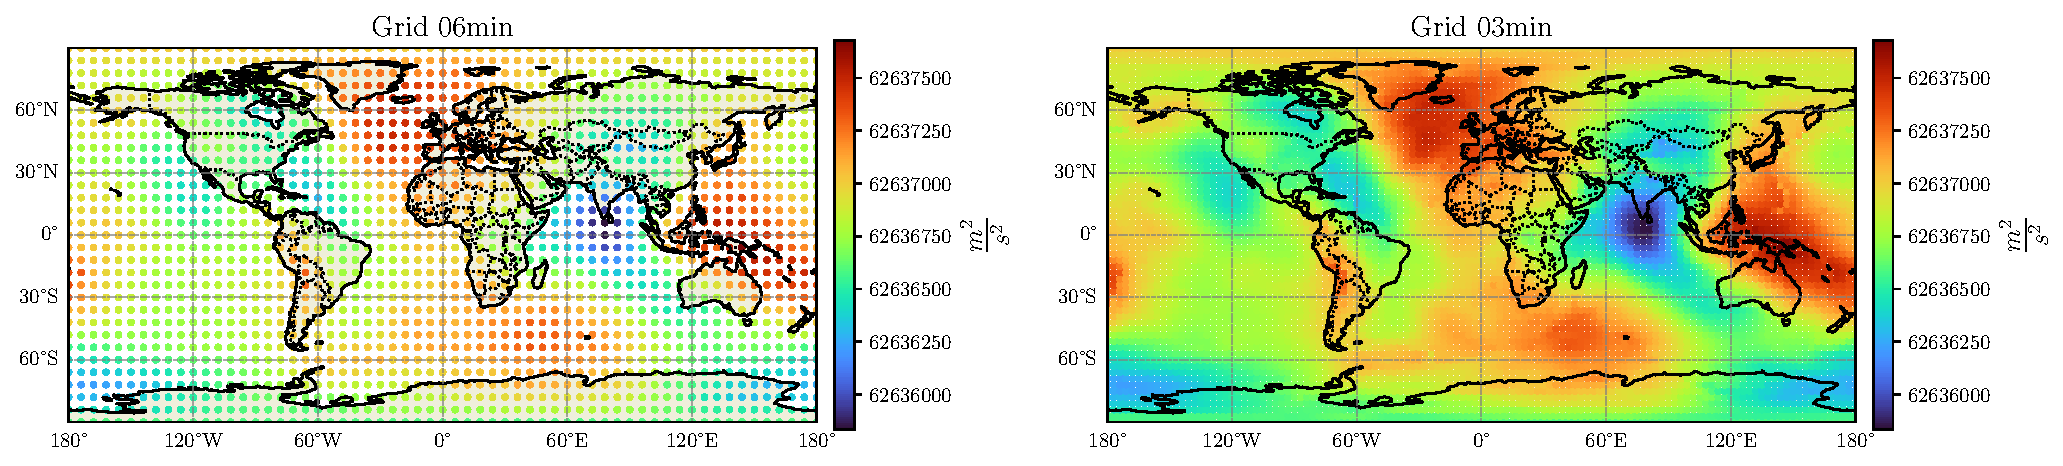
\includegraphics[width=16cm]{../Outputs/MainData.pdf}
		\caption{Gravity potential data used for interpolation and validation.}
		\label{fig:MainData}
	\end{figure}
	
	The design matrix $A$ for solving coefficients is ill-conditioned, with the condition number of $7.15*10^{49}$. The Picard plot for this matrix is shown in figure \ref{fig:PicardPlot}. 

	\begin{figure}[h!]
		\centering
		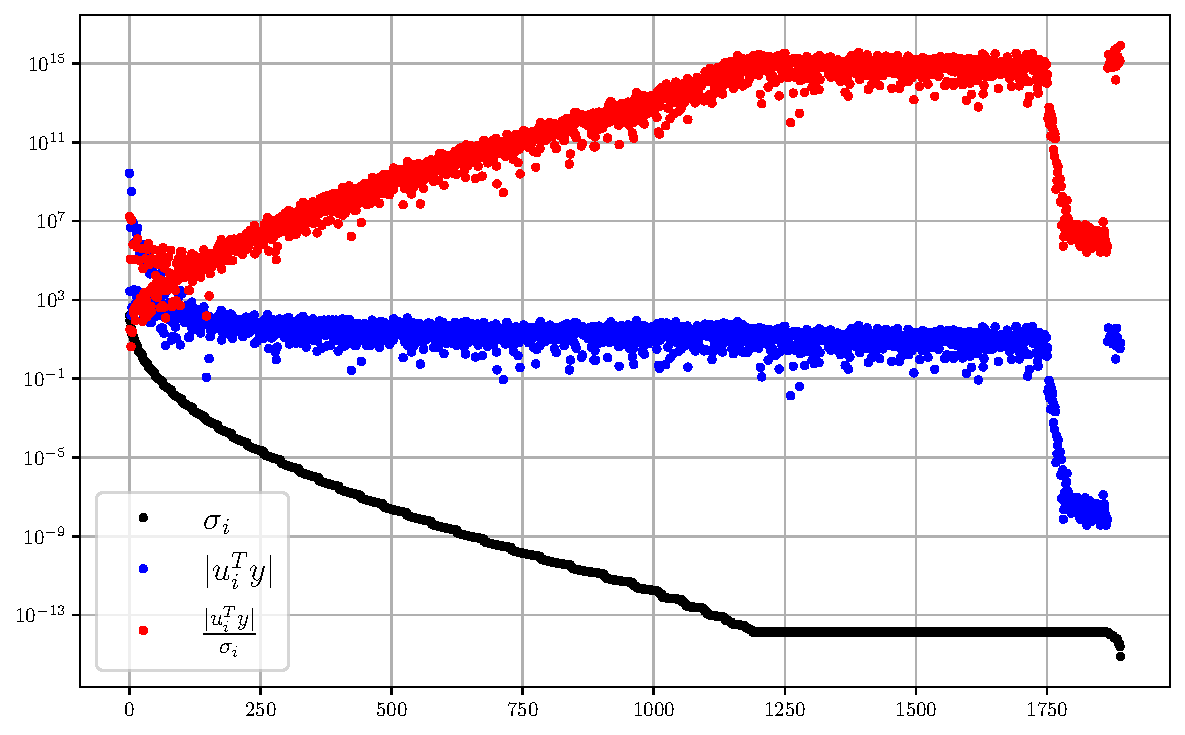
\includegraphics[height=3.8cm]{../Outputs/PicardPlot.pdf}
		\caption{Picard plot of the design matrix.}
		\label{fig:PicardPlot}
	\end{figure}
	
	Therefore methods of regularization is required for calculating the coefficients, and the solution by simply inverting the design matrix is not a reasonable solution, as shown in figure \ref{fig:NoRegResult}.  
	
	\begin{figure}[h!]
		\centering
		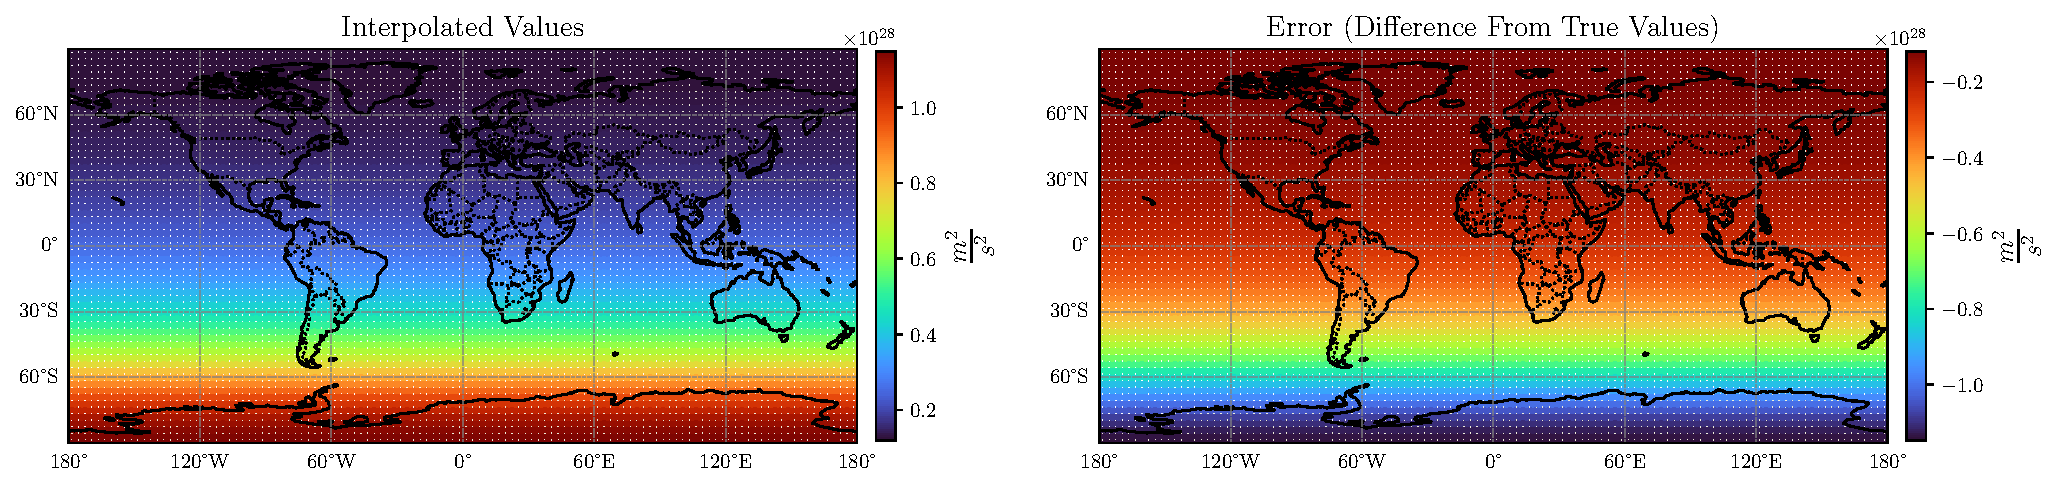
\includegraphics[width=15cm]{../Outputs/NoRegResult.pdf}
		\caption{Results without using regularization methods.}
		\label{fig:NoRegResult}
	\end{figure}
	
	Regularization methods used are TSVD and Tikhonov (With regularization parameter calculated from VCE). Cholesky decomposition is also used, which is a method for cases with numerical problems.
	
	Error of interpolation is defined as shown in equation \ref{eq:error}, Where $l$ is the true value acquired from XGM2019 model, and $\hat{l}$ is the interpolated value.
	
	\begin{equation}
		e = l - \hat{l}
		\label{eq:error}
	\end{equation}

	\section{Results}
	
	\subsection{Abel-Poisson}
	
	Results for Abel-Poisson kernel is shown in the figures \ref{fig:AbelPoisson_Chol} to \ref{fig:AbelPoisson_VCE}. The value of parameter $h$ for this kernel was considered 0.360. Mean and norm ($L_2$) of these three methods are shown in table \ref{tab:AbelPoisson_Error}.
	
	\begin{table}[h!]
		\centering
		\caption{Error for interpolation using Abel-Poisson kernel (unit of values are $\frac{m^2}{s^2}$).}
		\vspace{0.3cm}
		\renewcommand{\arraystretch}{1.4}
		\begin{tabular}{c|c|c|c}
			\textbf{Method} & Cholesky & TSVD & Tikhonov (VCE) \\
			\hline 
			\textbf{Mean Error} & 0.1612 & 0.1766 & -2.4909 \\
			\hline 
			\textbf{Norm of Errors} & 2014.1234 & 4175.8890 & 3931.1049 \\
		\end{tabular}
		\label{tab:AbelPoisson_Error}
	\end{table}
	
	\begin{figure}[h!]
		\centering
		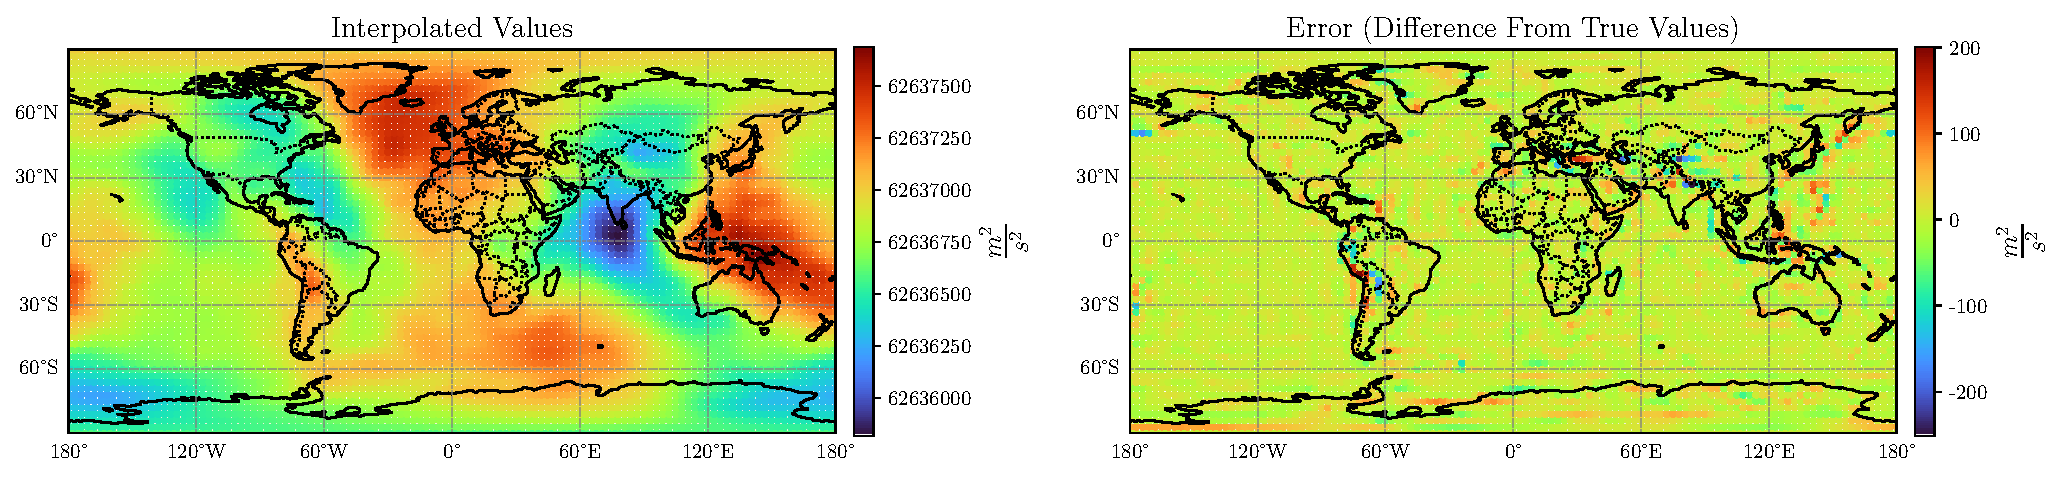
\includegraphics[width=16cm]{../Outputs/AbelPoisson_Cholesky.pdf}
		\caption{Results of Abel-Poisson kernel with Cholesky decomposition.}
		\label{fig:AbelPoisson_Chol}
	\end{figure}
	
	\begin{figure}[h!]
		\centering
		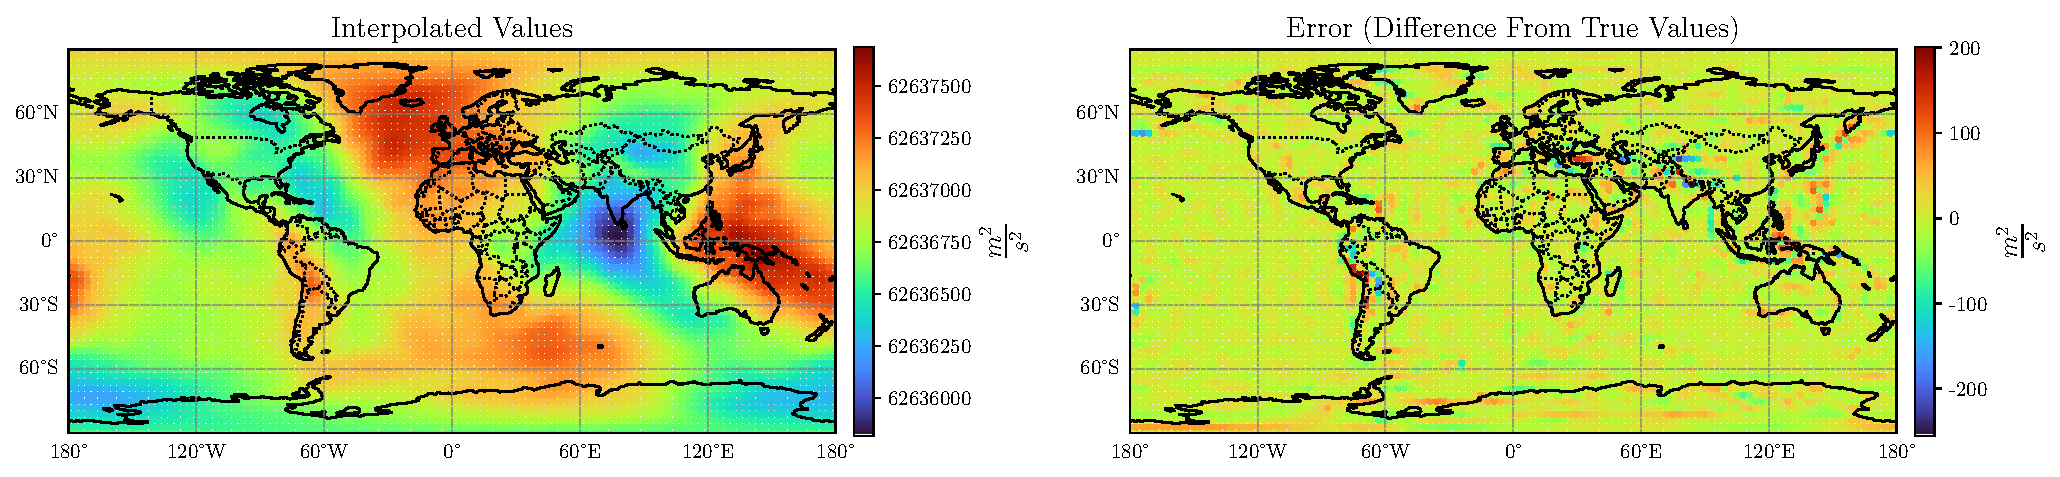
\includegraphics[width=16cm]{../Outputs/AbelPoisson_TSVD.pdf}
		\caption{Results of Abel-Poisson kernel with TSVD method.}
		\label{fig:AbelPoisson_TSVD}
	\end{figure}
	
	\begin{figure}[h!]
		\centering
		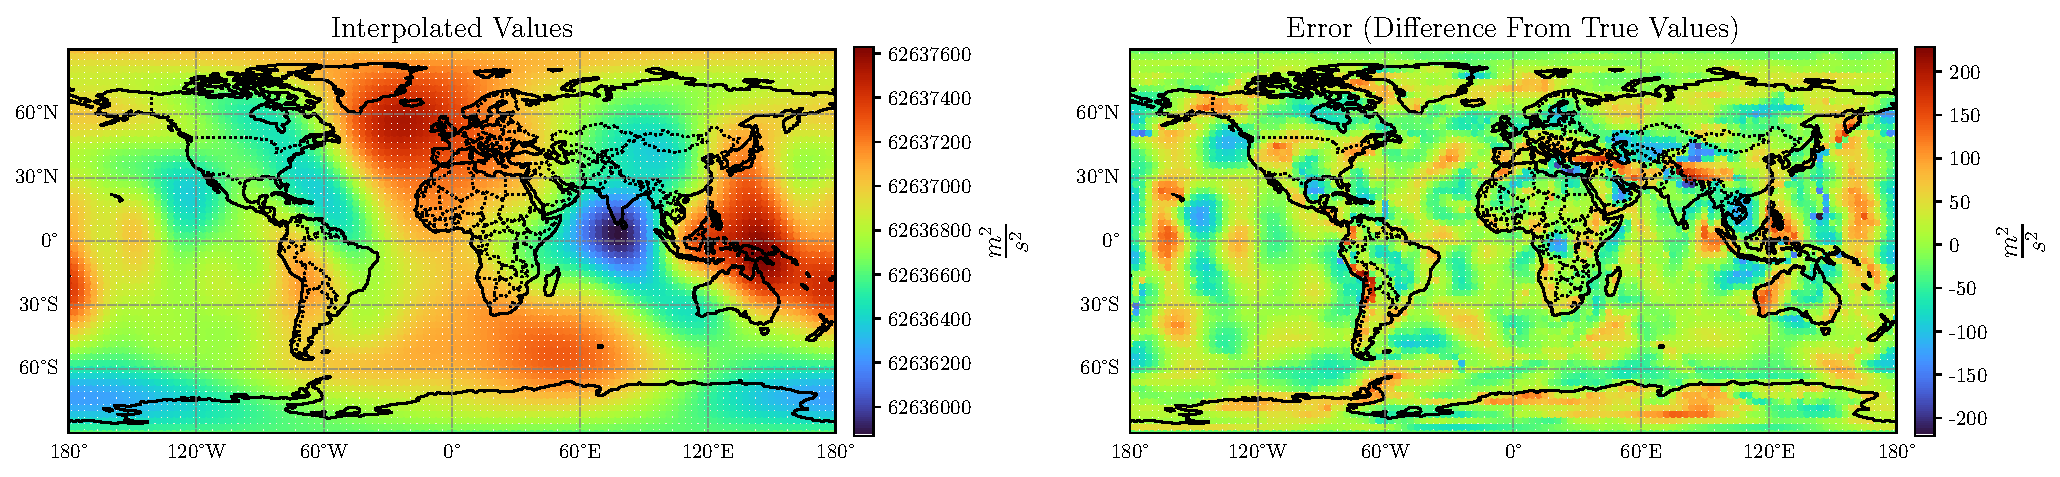
\includegraphics[width=16cm]{../Outputs/AbelPoisson_VCE.pdf}
		\caption{Results of Abel-Poisson kernel with Tikhonov (VCE) method.}
		\label{fig:AbelPoisson_VCE}
	\end{figure}
	
	
	
	\subsection{Singularity}
	
	Results for Singularity kernel is shown in the figures \ref{fig:Singularity_Chol} to \ref{fig:Singularity_VCE}. The value of parameter $h$ for this kernel was considered 0.405. Mean and norm ($L_2$) of these three methods are shown in table \ref{tab:Singularity_Error}.
	
	\begin{table}[h!]
		\centering
		\caption{Error for interpolation using Singularity kernel (unit of values are $\frac{m^2}{s^2}$).}
		\vspace{0.3cm}
		\renewcommand{\arraystretch}{1.4}
		\begin{tabular}{c|c|c|c}
			\textbf{Method} & Cholesky & TSVD & Tikhonov (VCE) \\
			\hline 
			\textbf{Mean Error} & 0.1814 & 0.1696 & 2.0778 \\
			\hline 
			\textbf{Norm of Errors} & 2014.3146 & 2016.4105 & 3931.1049 \\
		\end{tabular}
		\label{tab:Singularity_Error}
	\end{table}
	
	\begin{figure}[h!]
		\centering
		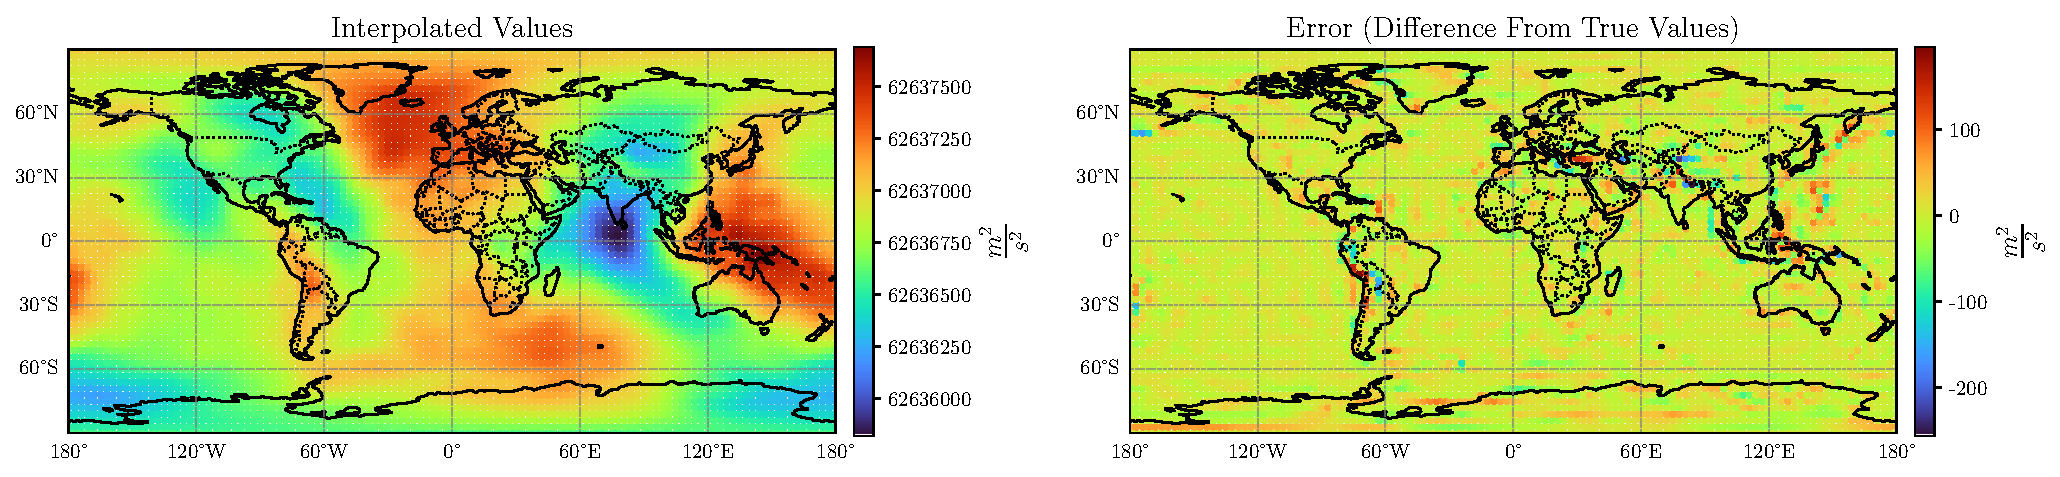
\includegraphics[width=16cm]{../Outputs/Singularity_Cholesky.pdf}
		\caption{Results of Singularity kernel with Cholesky decomposition.}
		\label{fig:Singularity_Chol}
	\end{figure}
	
	\clearpage
	
	\begin{figure}[h!]
		\centering
		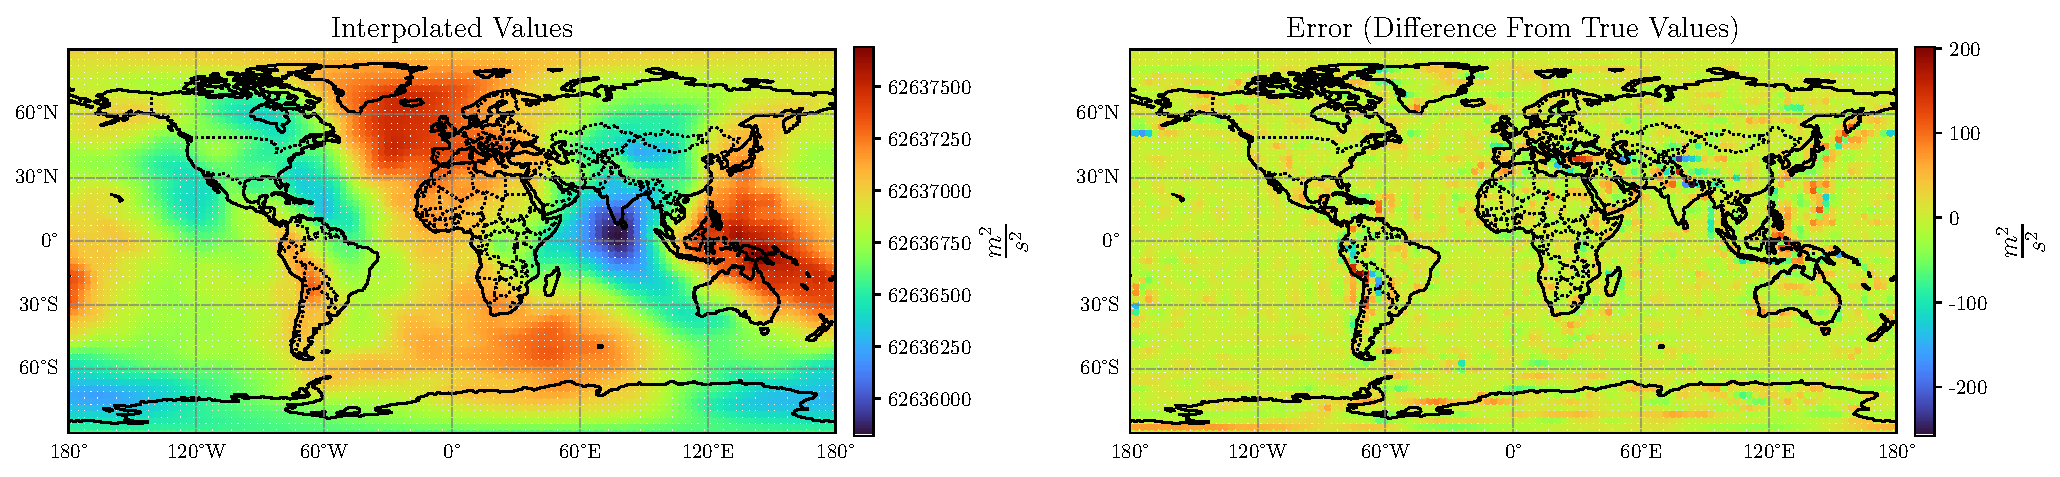
\includegraphics[width=16cm]{../Outputs/Singularity_TSVD.pdf}
		\caption{Results of Singularity kernel with TSVD method.}
		\label{fig:Singularity_TSVD}
	\end{figure}
	
	\begin{figure}[h!]
		\centering
		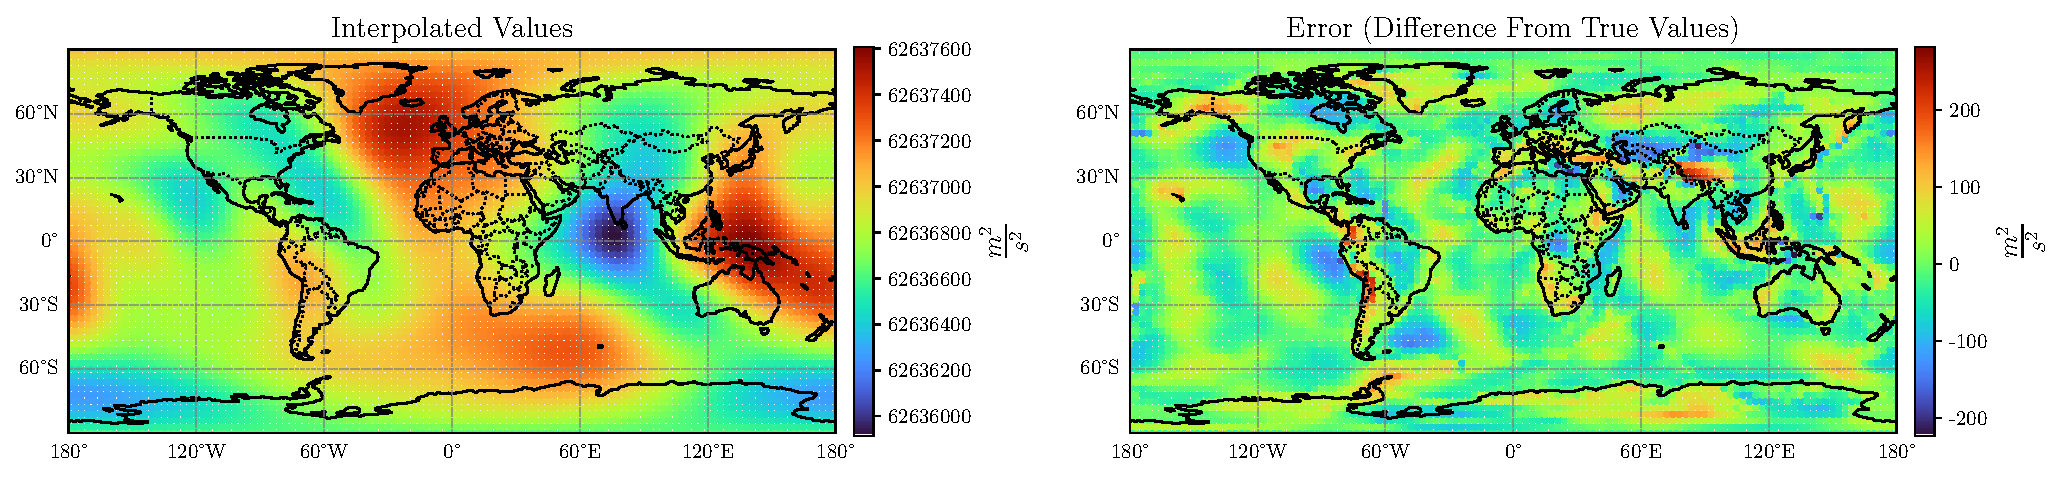
\includegraphics[width=16cm]{../Outputs/Singularity_VCE.pdf}
		\caption{Results of Singularity kernel with Tikhonov (VCE) method.}
		\label{fig:Singularity_VCE}
	\end{figure}
	
	
	\subsection{Logarithmic}
	
	Results for Singularity kernel is shown in the figures \ref{fig:Logarithmic_Chol} to \ref{fig:Logarithmic_VCE}. The value of parameter $h$ for this kernel was considered 0.457. Mean and norm ($L_2$) of these three methods are shown in table \ref{tab:Logarithmic_Error}.
	
	\begin{table}[h!]
		\centering
		\caption{Error for interpolation using Logarithmic kernel (unit of values are $\frac{m^2}{s^2}$).}
		\vspace{0.3cm}
		\renewcommand{\arraystretch}{1.4}
		\begin{tabular}{c|c|c|c}
			\textbf{Method} & Cholesky & TSVD & Tikhonov (VCE) \\
			\hline 
			\textbf{Mean Error} & 0.1503 & 0.1746 & 0.4764 \\
			\hline 
			\textbf{Norm of Errors} & 2005.1889 & 2013.2417 & 5436.0035 \\
		\end{tabular}
		\label{tab:Logarithmic_Error}
	\end{table}
	
	\begin{figure}[h!]
		\centering
		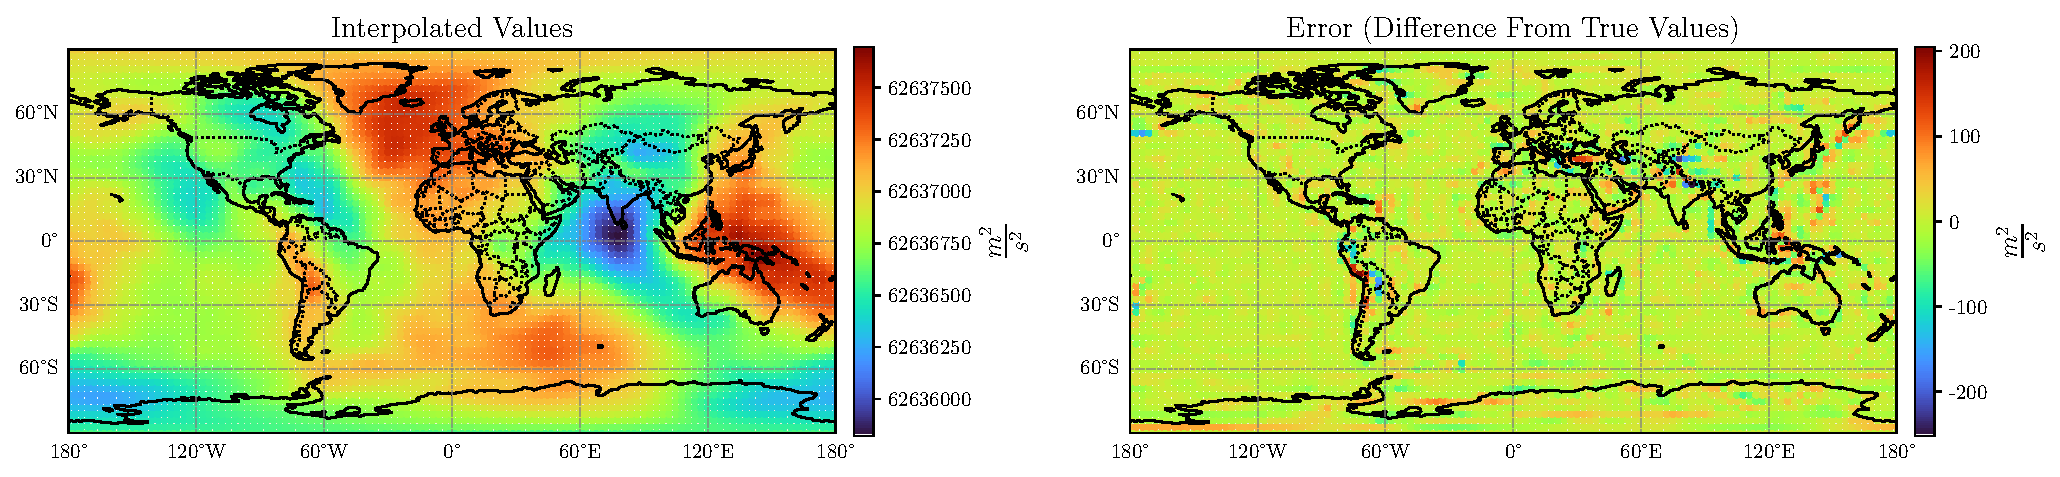
\includegraphics[width=16cm]{../Outputs/Logarithmic_Cholesky.pdf}
		\caption{Results of Logarithmic kernel with Cholesky decomposition.}
		\label{fig:Logarithmic_Chol}
	\end{figure}
	
	\begin{figure}[h!]
		\centering
		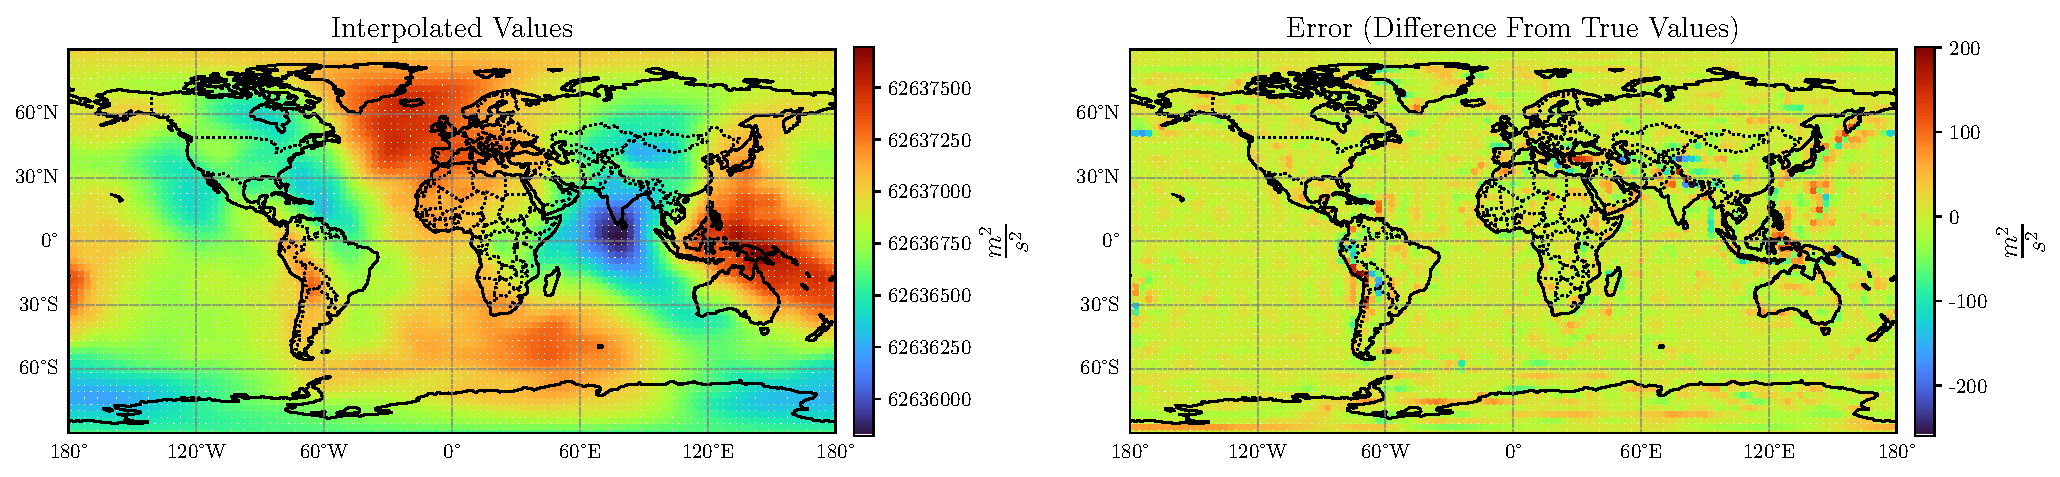
\includegraphics[width=16cm]{../Outputs/Logarithmic_TSVD.pdf}
		\caption{Results of Logarithmic kernel with TSVD method.}
		\label{fig:Logarithmic_TSVD}
	\end{figure}
	
	\begin{figure}[h!]
		\centering
		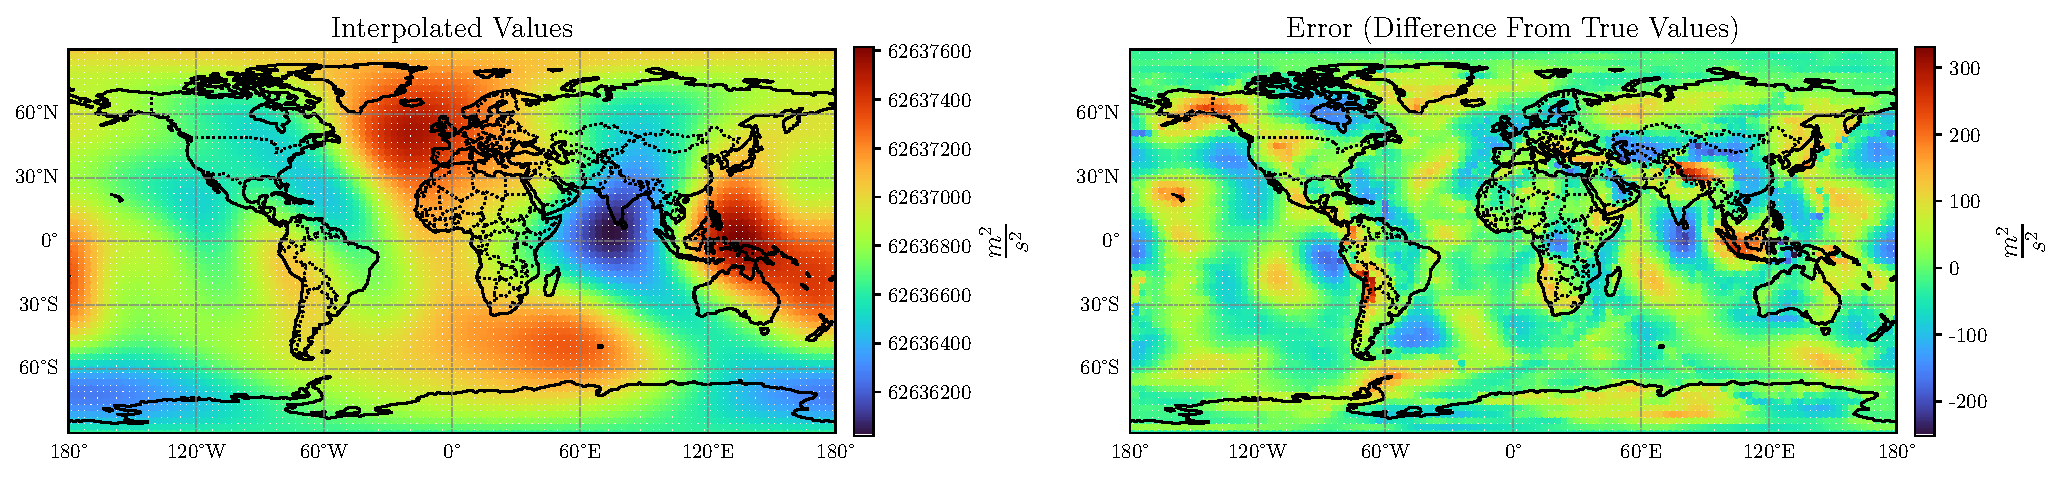
\includegraphics[width=16cm]{../Outputs/Logarithmic_VCE.pdf}
		\caption{Results of Logarithmic kernel with Tikhonov (VCE) method.}
		\label{fig:Logarithmic_VCE}
	\end{figure}

	
	\subsection{Abel-Poisson With Noise}
	
	In this case, white-noise with standard deviation of $200 \frac{m^2}{s^2}$ was added to the input values. Results are shown in the figures \ref{fig:AbelPoisson_Chol_Noise} to \ref{fig:AbelPoisson_VCE_Noise}.Also, mean and norm ($L_2$) of the three methods are shown in table \ref{tab:AbelPoisson_Error_Noise}.
	As it can be understood from results, by adding white-noise to the data, Cholesky and TSVD can not achieve satisfactory results. But Tikhonov method using VCE can have much realistic and smoother results that other two methods. 
	
	\begin{table}[h!]
		\centering
		\caption{Error for interpolation using Abel-Poisson kernel and added white-noise (unit of values are $\frac{m^2}{s^2}$).}
		\vspace{0.3cm}
		\renewcommand{\arraystretch}{1.4}
		\begin{tabular}{c|c|c|c}
			\textbf{Method} & Cholesky & TSVD & Tikhonov (VCE) \\
			\hline 
			\textbf{Mean Error} & -3.1558 & -3.1328 & 71.1711 \\
			\hline 
			\textbf{Norm of Errors} & 5548.1711 & 12137.6909 & 8200.7749 \\
		\end{tabular}
		\label{tab:AbelPoisson_Error_Noise}
	\end{table}

	\begin{figure}[h!]
		\centering
		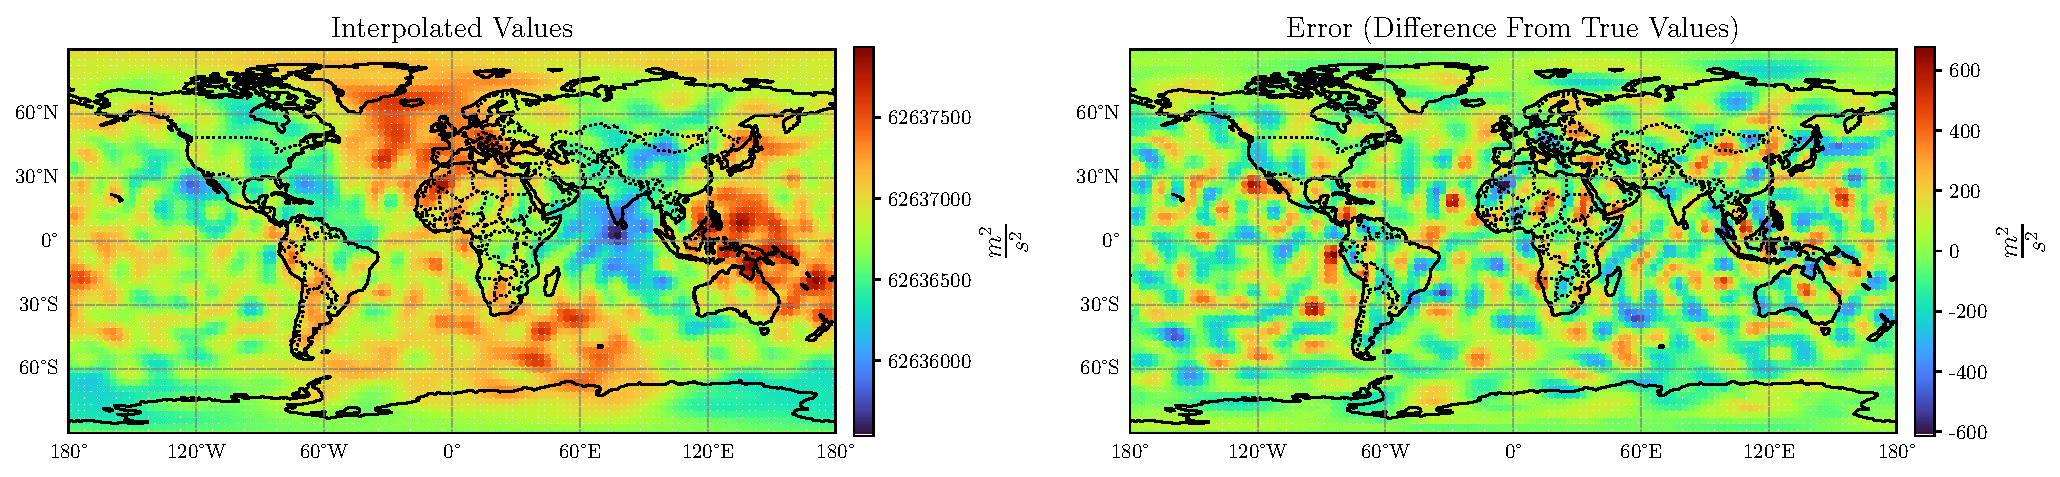
\includegraphics[width=16cm]{../Outputs/AbelPoisson_Cholesky_Noise.pdf}
		\caption{Results of Abel-Poisson kernel with Cholesky decomposition and added white-noise.}
		\label{fig:AbelPoisson_Chol_Noise}
	\end{figure}
	
	\clearpage
	
	\begin{figure}[h!]
		\centering
		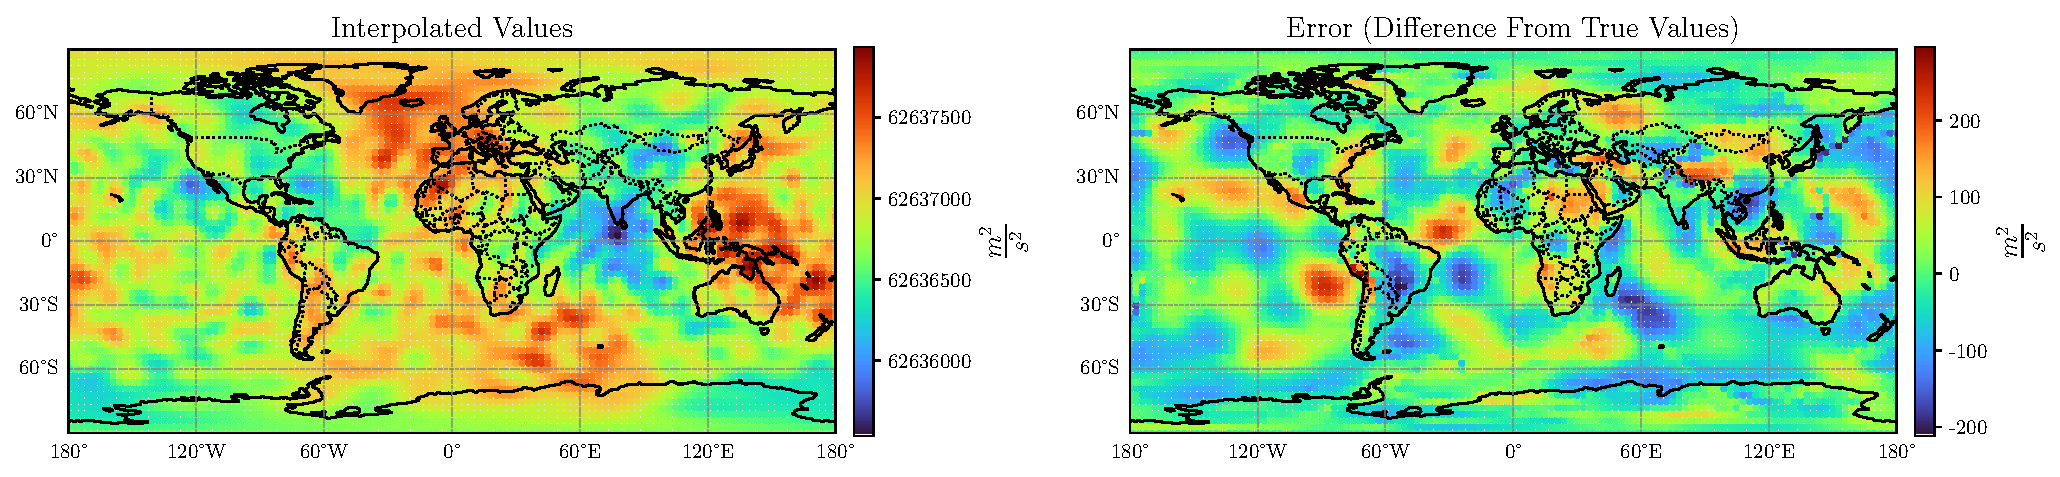
\includegraphics[width=16cm]{../Outputs/AbelPoisson_TSVD_Noise.pdf}
		\caption{Results of Abel-Poisson kernel with TSVD method and added white-noise.}
		\label{fig:AbelPoisson_TSVD_Noise}
	\end{figure}
	
	\begin{figure}[h!]
		\centering
		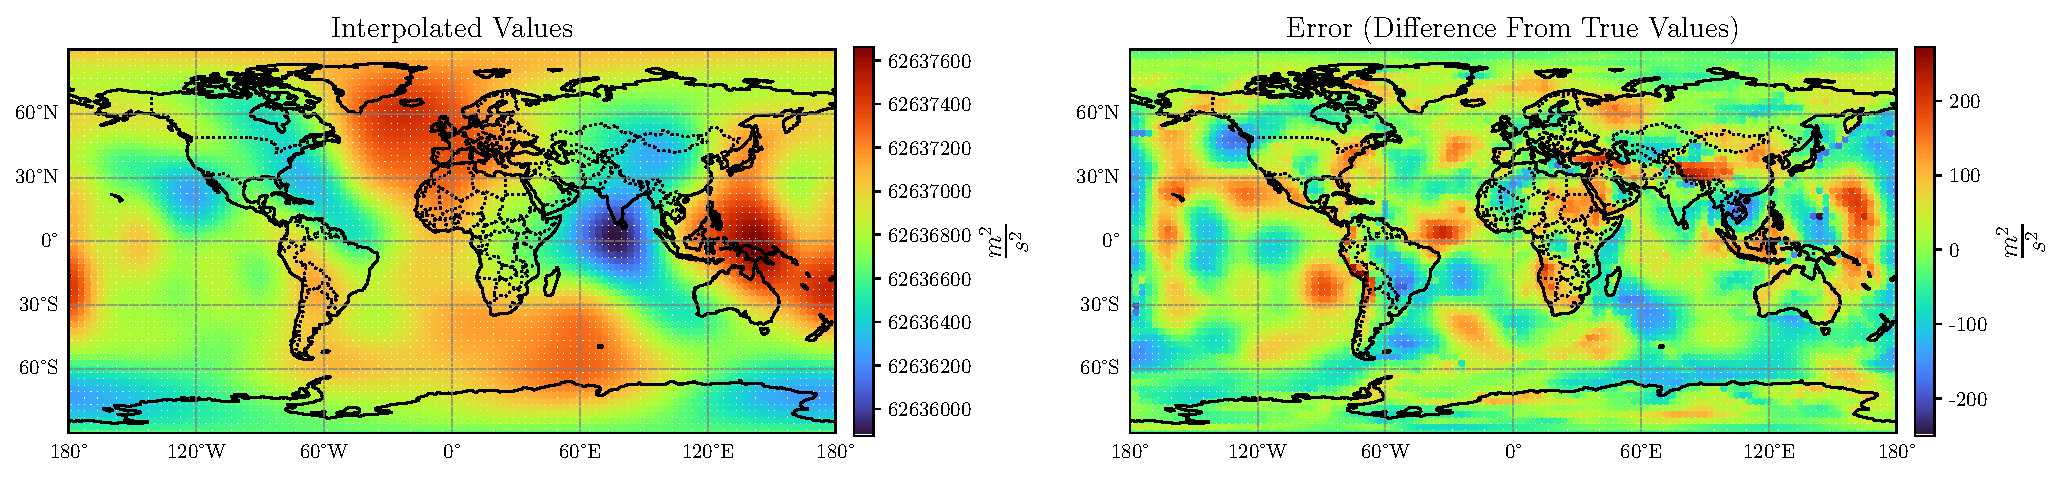
\includegraphics[width=16cm]{../Outputs/AbelPoisson_VCE_Noise.pdf}
		\caption{Results of Abel-Poisson kernel with Tikhonov (VCE) method and added white-noise.}
		\label{fig:AbelPoisson_VCE_Noise}
	\end{figure}
	
	
	\subsection{Singularity With Noise}
	
	The same amount of white-noise was added to the input values. Results are shown in the figures \ref{fig:Singularity_Chol_Noise} to \ref{fig:Singularity_VCE_Noise}.Also, mean and norm ($L_2$) of the three methods are shown in table \ref{tab:Singularity_Error_Noise}.
	
	\begin{table}[h!]
		\centering
		\caption{Error for interpolation using Singularity kernel and added white-noise (unit of values are $\frac{m^2}{s^2}$).}
		\vspace{0.3cm}
		\renewcommand{\arraystretch}{1.4}
		\begin{tabular}{c|c|c|c}
			\textbf{Method} & Cholesky & TSVD & Tikhonov (VCE) \\
			\hline 
			\textbf{Mean Error} & -8.9409 & -8.1949 & -7.2813 \\
			\hline 
			\textbf{Norm of Errors} & 12540.6580 & 5736.3606 & 5770.8221 \\
		\end{tabular}
		\label{tab:Singularity_Error_Noise}
	\end{table}
	
	\begin{figure}[h!]
		\centering
		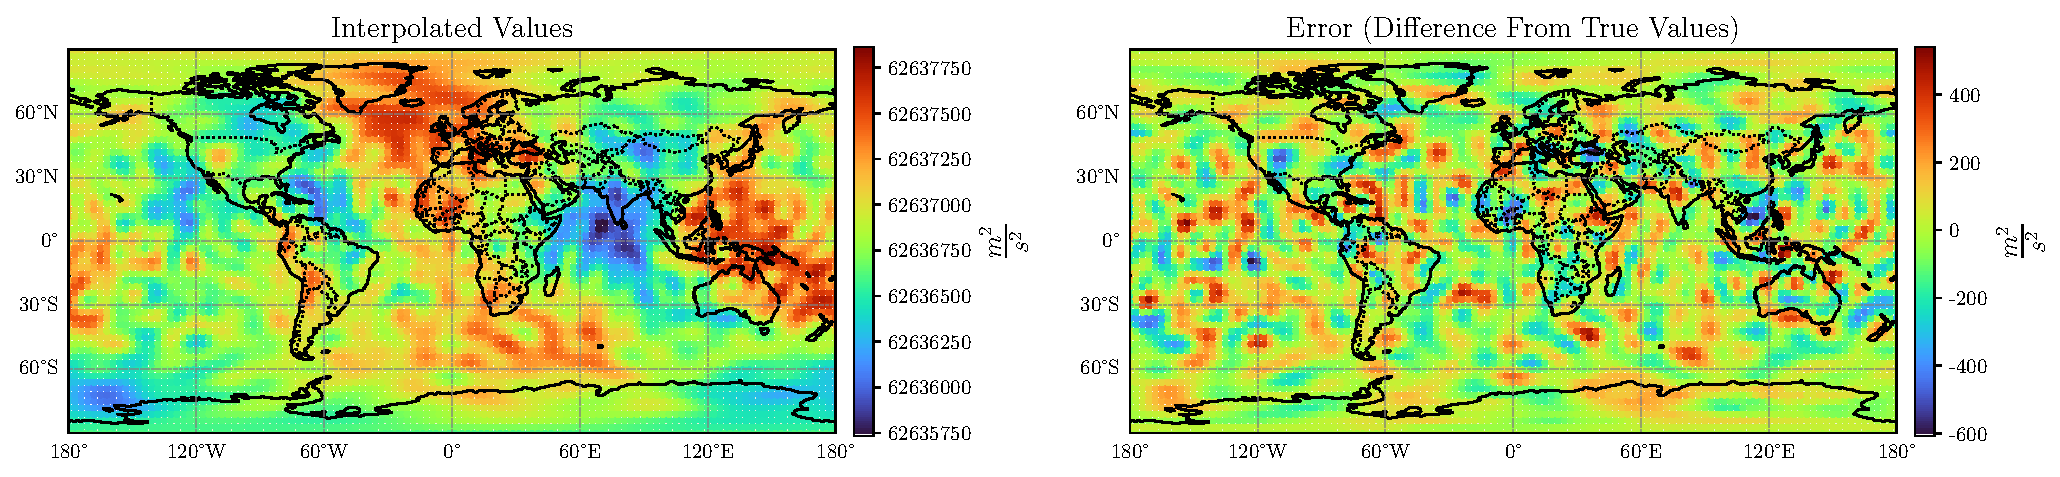
\includegraphics[width=16cm]{../Outputs/Singularity_Cholesky_Noise.pdf}
		\caption{Results of Singularity kernel with Cholesky decomposition and added white-noise.}
		\label{fig:Singularity_Chol_Noise}
	\end{figure}
	
	\clearpage
	
	\begin{figure}[h!]
		\centering
		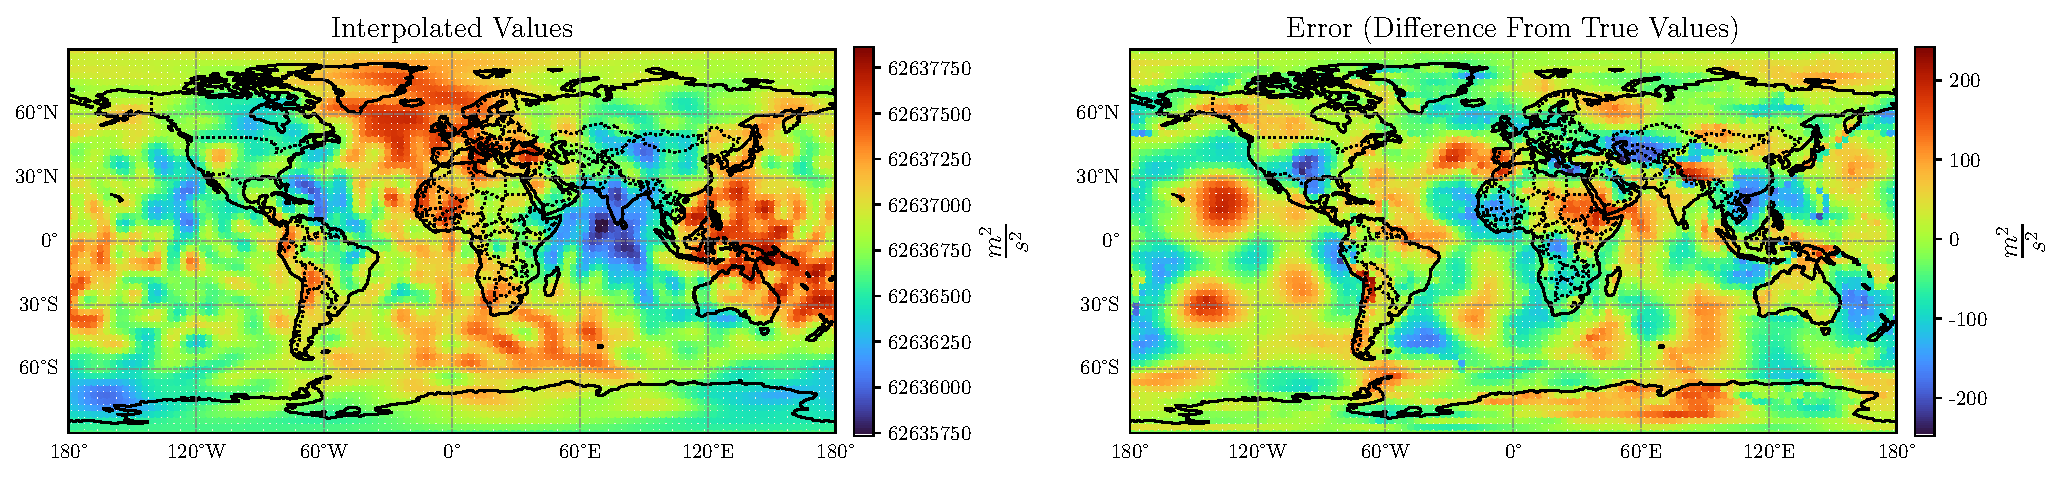
\includegraphics[width=16cm]{../Outputs/Singularity_TSVD_Noise.pdf}
		\caption{Results of Singularity kernel with TSVD method and added white-noise.}
		\label{fig:Singularity_TSVD_Noise}
	\end{figure}
	
	\begin{figure}[h!]
		\centering
		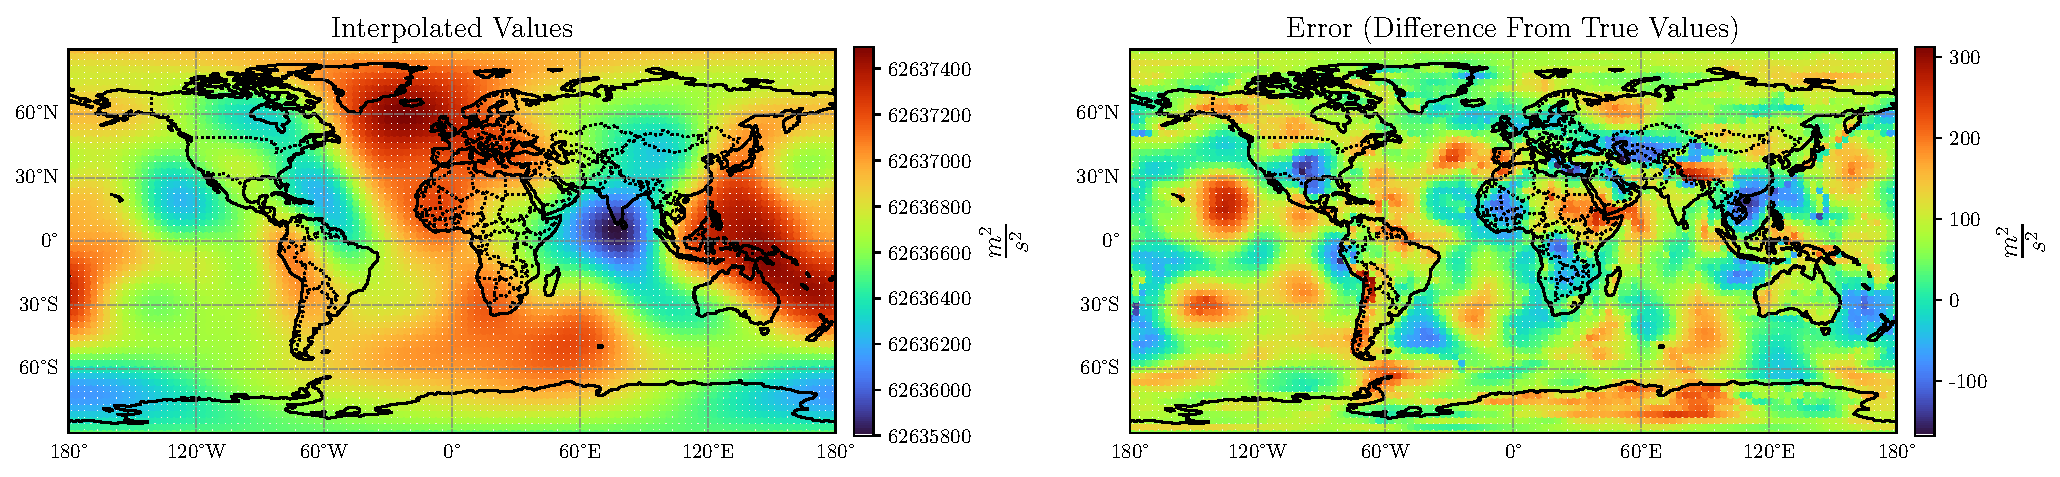
\includegraphics[width=16cm]{../Outputs/Singularity_VCE_Noise.pdf}
		\caption{Results of Singularity kernel with Tikhonov (VCE) method and added white-noise.}
		\label{fig:Singularity_VCE_Noise}
	\end{figure}


	\subsection{Logarithmic With Noise}
	
	Results are shown in the figures \ref{fig:Logarithmic_Chol_Noise} to \ref{fig:Logarithmic_VCE_Noise}.Also, mean and norm ($L_2$) of the three methods are shown in table \ref{tab:Logarithmic_Error_Noise}.
	
	\begin{table}[h!]
		\centering
		\caption{Error for interpolation using Logarithmic kernel and added white-noise (unit of values are $\frac{m^2}{s^2}$).}
		\vspace{0.3cm}
		\renewcommand{\arraystretch}{1.4}
		\begin{tabular}{c|c|c|c}
			\textbf{Method} & Cholesky & TSVD & Tikhonov (VCE) \\
			\hline 
			\textbf{Mean Error} & 7.5111 & 7.3757 & 74.2444 \\
			\hline 
			\textbf{Norm of Errors} & 5155.9012 & 12404.6648 & 8167.3250 \\
		\end{tabular}
		\label{tab:Logarithmic_Error_Noise}
	\end{table}
	
	\begin{figure}[h!]
		\centering
		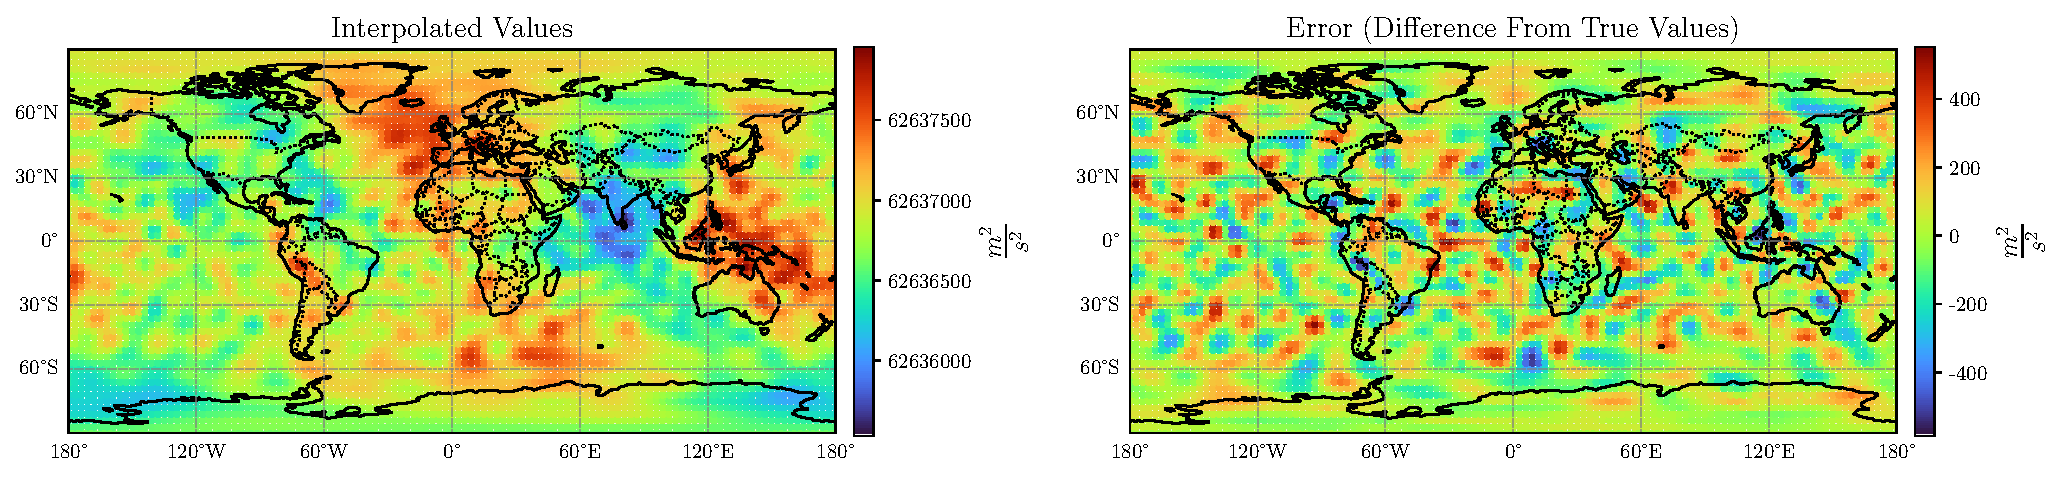
\includegraphics[width=16cm]{../Outputs/Logarithmic_Cholesky_Noise.pdf}
		\caption{Results of Logarithmic kernel with Cholesky decomposition and added white-noise.}
		\label{fig:Logarithmic_Chol_Noise}
	\end{figure}
	
	\clearpage
	
	\begin{figure}[h!]
		\centering
		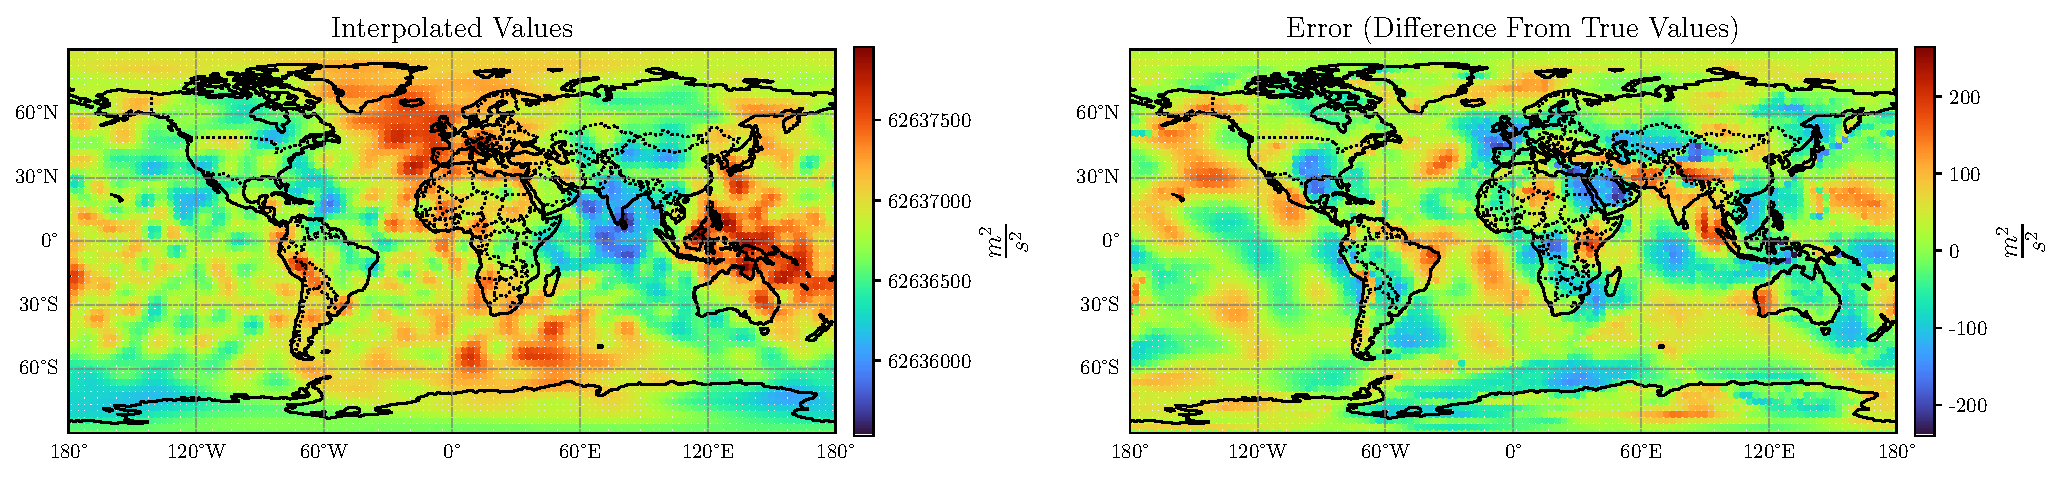
\includegraphics[width=16cm]{../Outputs/Logarithmic_TSVD_Noise.pdf}
		\caption{Results of Logarithmic kernel with TSVD method and added white-noise.}
		\label{fig:Logarithmic_TSVD_Noise}
	\end{figure}
	
	\begin{figure}[h!]
		\centering
		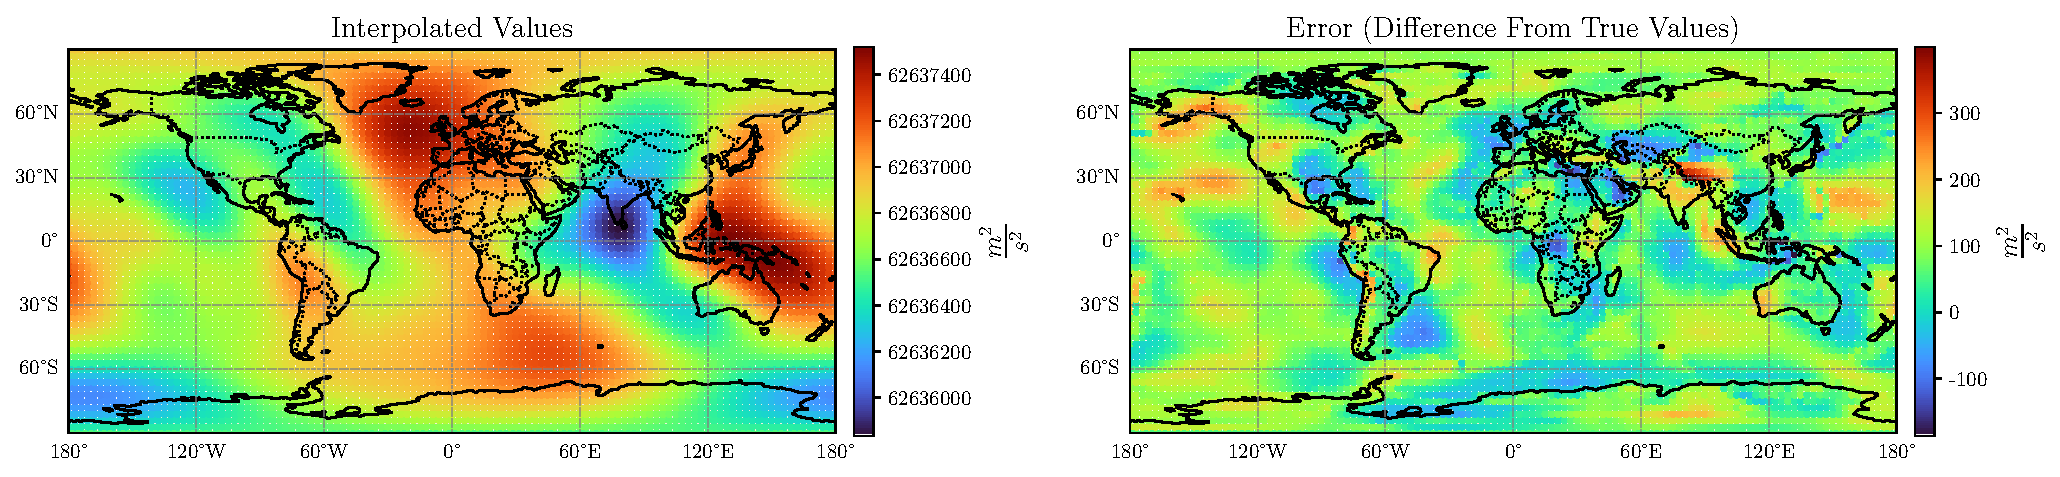
\includegraphics[width=16cm]{../Outputs/Logarithmic_VCE_Noise.pdf}
		\caption{Results of Logarithmic kernel with Tikhonov (VCE) method and added white-noise.}
		\label{fig:Logarithmic_VCE_Noise}
	\end{figure}
	
\end{document}
